\chapter{Audio Emotion Detection}

This chapter examines the audio emotion recognition component of the multimodal framework, focusing on the use of IBM Watson's capabilities. The analysis includes performance tests to assess the accuracy and speed of IBM Watson in detecting emotions from audio input. Additionally, this chapter discusses the role of large language models (LLMs) in the context of emotion recognition and the limitations that prevent the use of OpenSMILE for this project. Through a detailed evaluation, this chapter aims to provide insight into the effectiveness of IBM Watson as an audio emotion recognition tool and the considerations involved in choosing appropriate technologies for audio analysis.

\section{IBM Watson}

Given the current computational demands of core functionalities and concurrent facial emotion recognition processes, it would be beneficial to consider offloading speech emotion recognition to an external entity. Using cloud-based solutions, such as IBM Watson's API, presents an appealing option. By interfacing with Watson, recorded human speech can be remotely processed, allowing emotional predictions based on textual analysis. This approach not only reduces the computational burden on the robot, but also harnesses the advanced emotion analysis capabilities offered by cloud services.

IBM Watson is a cognitive computing platform developed by IBM that uses artificial intelligence (AI) techniques to analyse and interpret large amounts of data. It includes a range of AI-powered services and tools designed to help businesses gain insights, make informed decisions, and improve user experiences in various industries. Watson's capabilities include natural language processing, machine learning, and data analytics, making it a versatile solution for addressing complex challenges.

One useful feature of IBM Watson is its conversational abilities, which allow for structured dialogue between the robot and the user. By integrating Watson's Conversation service, the robot can engage in structured conversations with users, responding to prompts and queries based on predefined conversation trees. This approach allows the robot to guide the conversation along predetermined paths, collecting specific information, or addressing user inquiries within predefined topics.

Ultimately, the choice to use cloud-based emotion recognition is a strategic decision that weighs computational efficiency against the aim of developing a flexible and emotionally intelligent robotic system. By tapping into external resources, we not only enhance the robot's performance but also pave the way for integrating state-of-the-art emotion analysis capabilities into the HRI framework, thereby enhancing the user experience and pushing the boundaries of human-robot interaction. \cite{Kumar2022-gd}

Initially, a system was created to incorporate IBM Watson as a chatbot to inform people about ongoing public health issues. The goal was to provide accurate and up-to-date responses to common questions and to give people peace of mind. The system was designed to use IBM’s sentiment analysis to detect fear and point people to resources that could help them. In addition, the chatbot provided the ability to connect an Aldebaran robot, which provided a physical presence that people could interact with. The robot would use its microphones to pick up user speech, which could then be sent to IBM for analysis, after which the robot would respond with what IBM Watson sent back. 

\begin{figure}[!htb]
    \centering 
    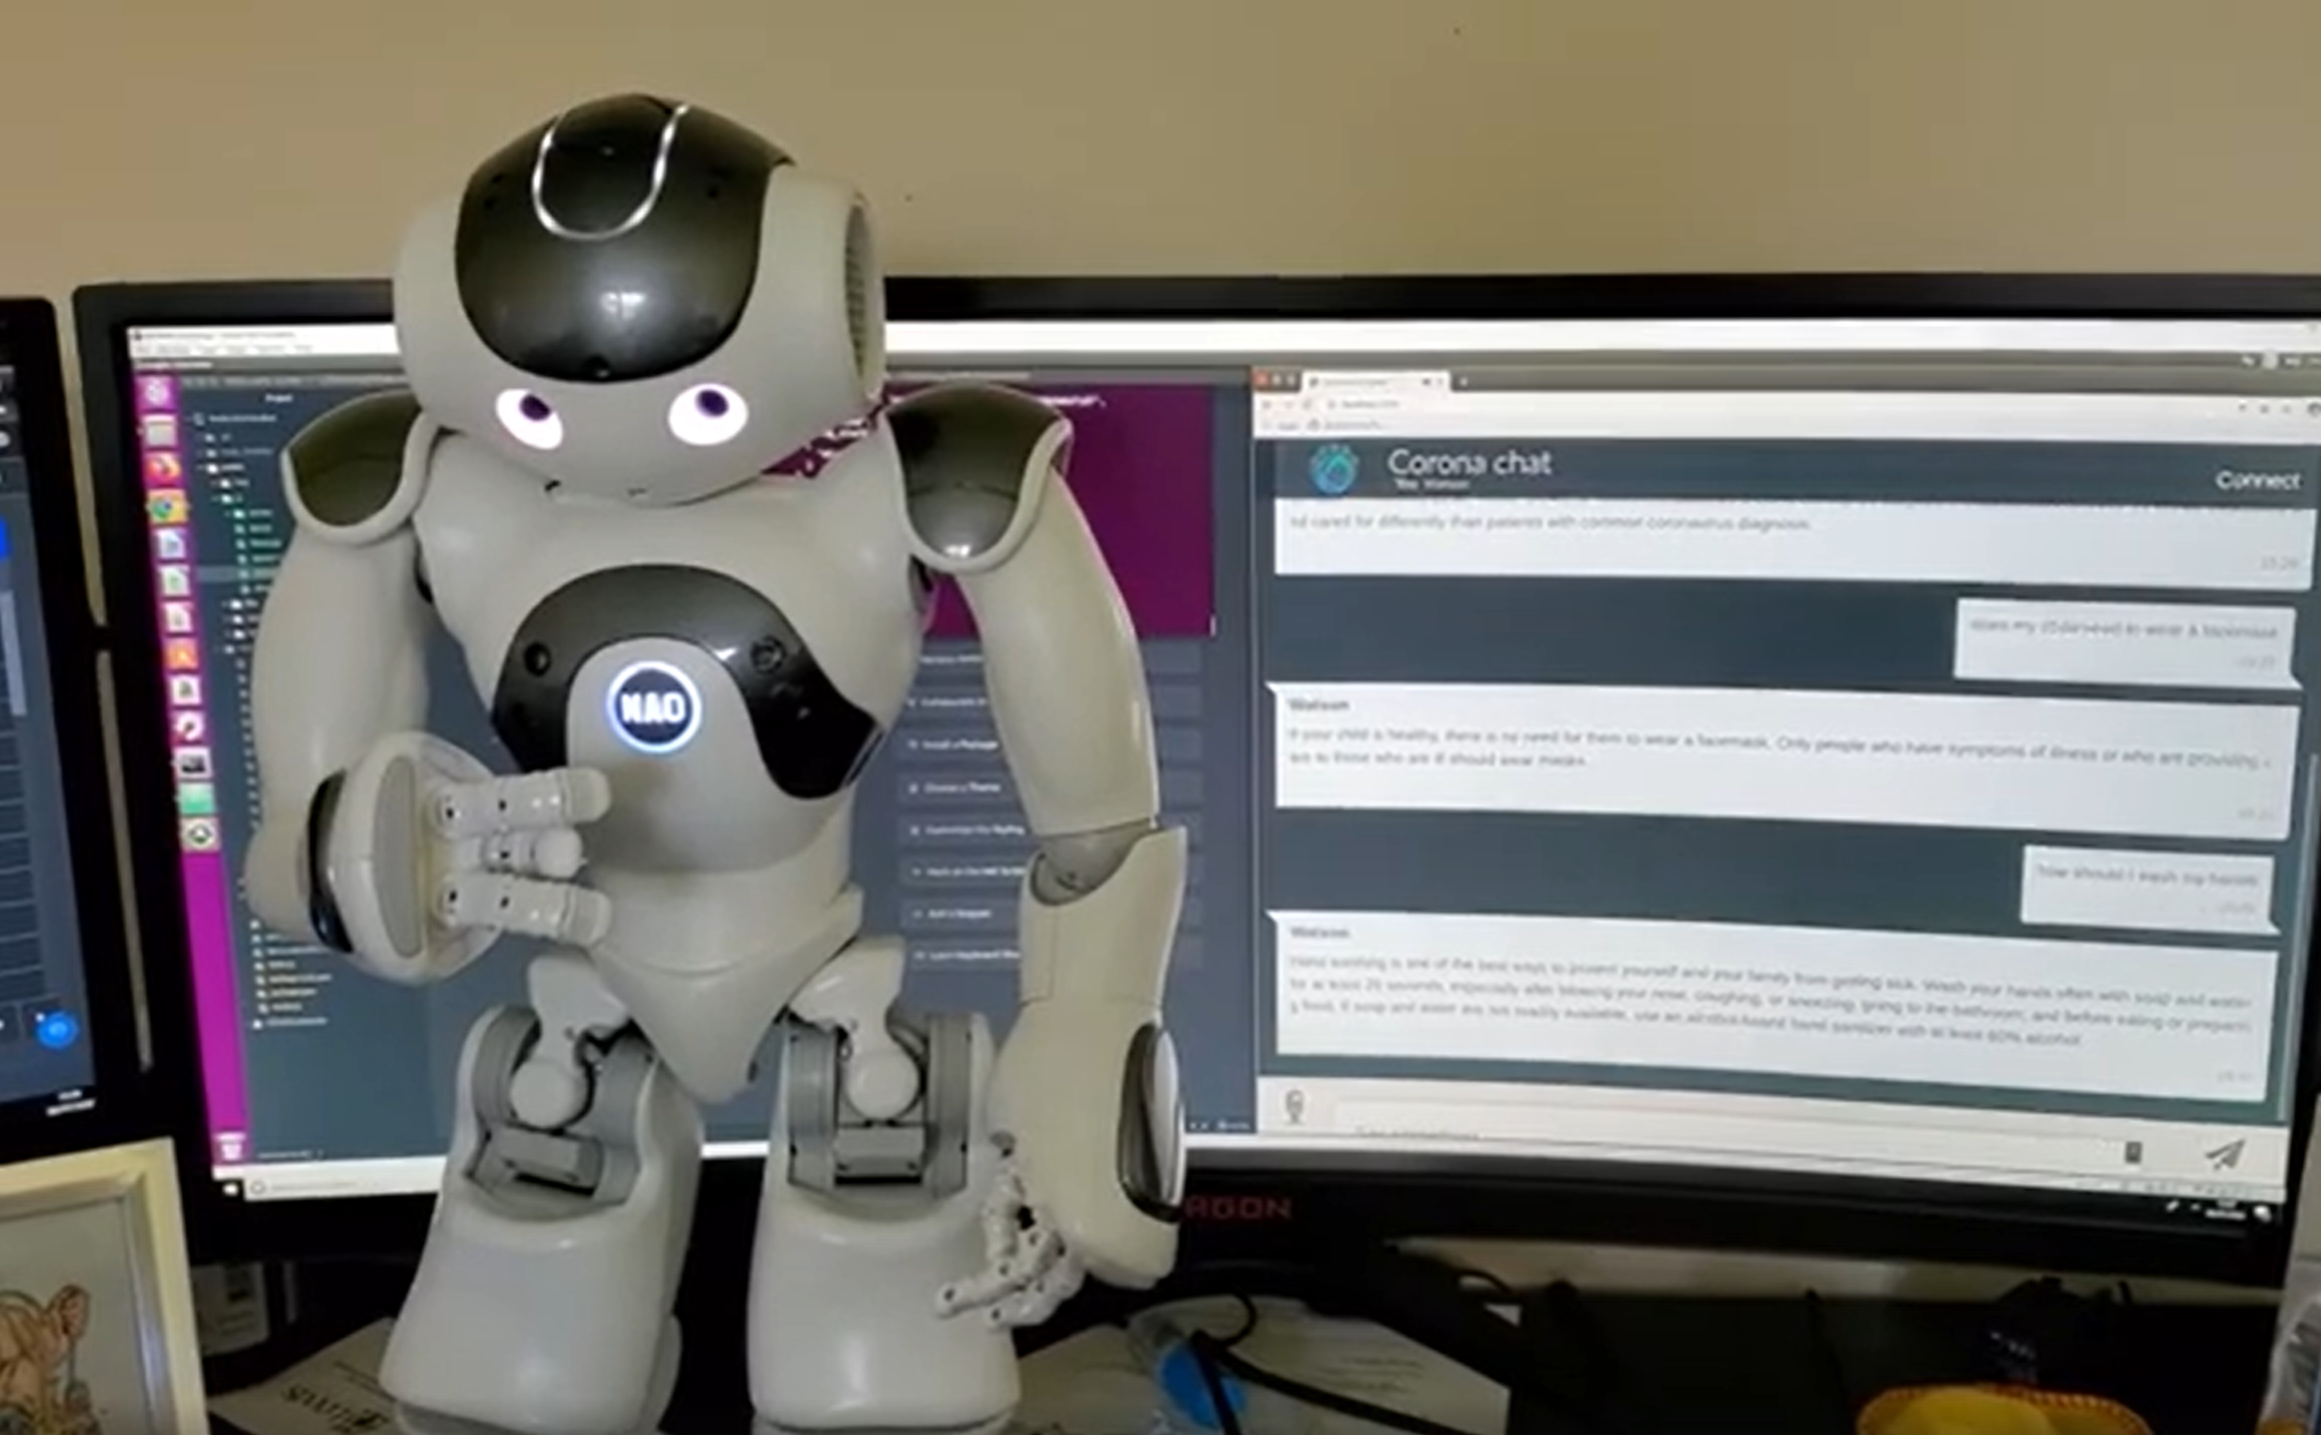
\includegraphics[scale=0.25]{aed_images/nao_with_chatbot.png}
    \caption{Aldebaran robot Nao with IBM Watson ChatBot}
    \label{figure:naochatbot}
\end{figure}

This system also leveraged IBM Watson's text-to-speech capabilities, allowing users to fully customise the generated voice based on a variety of parameters. In addition to selecting the gender of the voice, users could choose accents from different regions, making the interaction more personalised and culturally relevant. This also allows adjustments to pitch, enabling a higher or lower tone depending on user preference or specific application needs.

\section{LLM}

It is important to note that while IBM Watson's Conversation service provides a structured approach to dialogue management, it may lack the spontaneity and flexibility of natural human conversation. Relying on conversation trees imposes constraints on the flow of interaction, limiting the opportunity for open-ended dialogue and real-time adaptation to user input. As a result, interactions with the robot may feel scripted or constrained, potentially detracting from the overall user experience in certain situations.

To achieve a natural and engaging human-robot interaction, it is imperative to develop a comprehensive system that integrates a Large Language Model (LLM). ChatGPT, a state-of-the-art language model, plays a crucial role in enabling seamless human-like conversations between the robot and the user \cite{chatgpt}. Its ability to generate contextually relevant responses allows for a more natural dialogue exchange that closely resembles human conversation patterns.

By incorporating ChatGPT into this system, we can create a more interactive and emotionally responsive dialogue experience. In this setup, the speech-emotion recognition system handles the analysis of user speech to detect emotions such as happiness, sadness, anger, or neutrality. These detected emotional states can then be communicated to ChatGPT alongside the text of the user's speech. This allows ChatGPT to factor in both the content of the conversation and the emotional context provided by the speech-emotion recognition system, helping it generate more empathetic and contextually appropriate responses.

For example, if the speech-emotion recognition system detects frustration in the user's voice, this emotional information can be fed to ChatGPT, allowing it to adapt its responses in real time to address the user’s emotional state more sensitively. This synergy allows for a deeper and more emotionally aware interaction, where ChatGPT can tailor the flow of the conversation based on both the user’s words and their emotional tone.

Additionally, ChatGPT can use the emotional feedback from the speech-emotion system to adjust the direction of the conversation, perhaps steering toward topics that might alleviate negative emotions or enhance positive ones. This makes it possible to create a more engaging and emotionally intelligent interaction, where the robot can respond in a way that feels more human and responsive to the user's mood. Using ChatGPT for dialogue and the emotion recognition system for emotional analysis, we enable a hybrid approach where each component focuses on its strengths, resulting in a more robust and user-centric interaction.

Thus, ChatGPT was integrated into the system. This allows users to interact with ChatGPT seamlessly through a browser, making it accessible from virtually any device, whether a desktop, laptop, or mobile device. This integration ensures that users can engage with the system without the need for specialised software or hardware, broadening its utility and accessibility. The Web Messenger supports both text- and speech-based interactions allowing the user to converse with the robot in a natural way.

One of the core strengths of this system lies in how it expands ChatGPT's capabilities, making it a far more versatile assistant. Using the function-calling mechanism, ChatGPT can now fetch real-time data such as weather reports, time, and date, or even retrieve specific data from databases. This transforms it from being a static question-answering system to an interactive, real-time assistant. Moreover, the system has been designed to allow future scalability, enabling developers to integrate additional functions based on evolving user needs, such as connecting to more advanced AI models, adding new APIs, or enhancing its conversational context-awareness.

The system could also leverage locally run language models, such as GPT4All, to enhance its natural language understanding and response capabilities. Running these models locally ensures full control over data privacy and security. This approach allows for greater flexibility, as the models can be fine-tuned to better suit the system's specific needs without reliance on external cloud services. In addition, the system can operate independently of an internet connection, making it more reliable in environments with limited or unstable connectivity. This setup offers both customisation options and scalability, ensuring robust performance for complex, language-driven tasks.

\section{OpenSMILE}

OpenSMILE \cite{opensmile-2010}, which stands for "Open-Source Speech and Music Interpretation by Large-Space Extraction", is a powerful open-source toolkit widely used in audio signal processing. Its primary function is to extract an extensive range of acoustic features from audio signals, providing a versatile platform for various applications that include speech recognition, emotion recognition, speaker identification, and music analysis. One of the key strengths of OpenSMILE lies in its modular architecture, which allows the customisation of the feature extraction process to suit specific requirements. This modularity is achieved through a collection of feature extraction components known as "functionals," each responsible for computing a particular set of features. It is possible to choose from a rich library of functionals and combine them as needed to create tailored feature sets.

Moreover, OpenSMILE is designed for real-time processing of audio streams, making it suitable for applications that demand low-latency feature extraction, such as real-time speech recognition systems or interactive multimedia applications. Its cross-platform compatibility ensures that it can seamlessly integrate into various environments running on major operating systems, including Windows, macOS, and Linux. Additionally, the toolkit offers extensive configuration options that allow one to specify parameters such as frame size, overlap, and feature selection, thus providing flexibility to adapt to various audio processing tasks.

OpenSMILE facilitates the integration of extracted features with machine learning algorithms, serving as a crucial preprocessing step for tasks such as classification. The features computed by OpenSMILE capture essential characteristics of audio signals, enabling accurate modelling and interpretation of audio data. However, given the limited resources available on a robotic platform, it could run into performance issues that severely limit its capabilities. The memory requirements of OpenSMILE can also be significant, particularly when extracting a large number of features from lengthy audio streams, with each feature set taking up to 100MB for a short 18-second audio clip. Robotics platforms typically have limited memory capacity, and allocating resources to OpenSMILE may strain the system, potentially impacting overall system stability and reliability. This limitation is purely hardware based and future robots that can afford more powerful systems would be able to utilise OpenSMILE feature extraction plus a classification model to determine emotions.

\section{IBM Waston Performance}

In this section, the performance of IBM Watson's Natural Language Understanding (NLU) service is evaluated in analysing the emotional content of various phrases. To ensure a robust assessment, each phrase was tested five times, and response times were recorded. The table \ref{tab:phrase_tests} presents the response times (in seconds) for each test run with ten different phrases shown in \ref{tab:phrases_emotions}.

\begin{table}[h!]
\centering
\caption{Phrases and their expected emotions}
\begin{tabular}{|p{9cm}|c|}
\hline
\textbf{Text} & \textbf{Expected Emotion} \\ \hline
I am so happy today! Everything is going great. & Joy \\ \hline
I am very sad and disappointed by the news. & Sadness \\ \hline
I am so angry at the situation! & Anger \\ \hline
This is so scary and frightening. & Fear \\ \hline
I am just so disgusted by what happened. & Disgust \\ \hline
The sun is shining and the birds are singing. It's a beautiful day to be alive. I feel so grateful for all the wonderful things in my life. I have a loving family, great friends, and a job that I am passionate about. Days like today make me feel like all the hard work has paid off and I can truly appreciate the beauty of life. & Joy \\ \hline
Today I received some heartbreaking news. A dear friend of mine passed away unexpectedly. The shock and sorrow I feel are overwhelming. We had so many plans together, so many dreams left unfulfilled. It's hard to imagine life without them. This loss leaves a void that can never be filled. & Sadness \\ \hline
I am furious about the latest policy changes at work. They were implemented without any consultation with the staff, and they make our jobs much harder. It feels like management doesn't care about our well-being or input. This kind of disregard is unacceptable, and I won't stand for it. & Anger \\ \hline
Walking through the dark alley, I could feel my heart racing. Every sound seemed amplified, and the shadows looked like they were moving. I couldn't shake the feeling that someone was following me. It was one of the most terrifying experiences I've ever had. I just wanted to get out of there as quickly as possible. & Fear \\ \hline
The food at that restaurant was absolutely disgusting. The meat was undercooked, the vegetables were soggy, and there was a strange smell coming from the kitchen. I felt nauseous just being there. It's unacceptable to serve such poor quality food to customers. & Disgust \\ \hline
\end{tabular}
\label{tab:phrases_emotions}
\end{table}
\clearpage

\begin{table}[h!]
\centering
\caption{Test results for IBM Watson's response times on 10 phrases across 5 runs in seconds, alongside the average time and standard deviation. The phrases in this table match the phrases in table \ref{tab:phrases_emotions} in order.}
\begin{tabular}{|c|c|c|c|c|c|c|c|}
\hline
\textbf{Test number} & \textbf{Run 1} & \textbf{Run 2} & \textbf{Run 3} & \textbf{Run 4} & \textbf{Run 5} & \textbf{Average} & \textbf{SD} \\ \hline
\textbf{Phrase 1}    & 1.81 & 2.07 & 1.36 & 1.58 & 1.45 & 1.654 & 0.257        \\ \hline
\textbf{Phrase 2}    & 0.69 & 0.51 & 0.38 & 0.40 & 0.36 & 0.468 & 0.123        \\ \hline
\textbf{Phrase 3}    & 0.43 & 0.47 & 0.39 & 0.36 & 0.40 & 0.41 &  0.037       \\ \hline
\textbf{Phrase 4}    & 0.69 & 0.63 & 0.38 & 0.39 & 0.43 & 0.504 & 0.130        \\ \hline
\textbf{Phrase 5}    & 0.38 & 0.38 & 0.40 & 1.23 & 0.48 & 0.574 & 0.330        \\ \hline
\textbf{Phrase 6}    & 0.47 & 0.40 & 0.60 & 0.52 & 0.43 & 0.484 & 0.071        \\ \hline
\textbf{Phrase 7}    & 0.56 & 0.43 & 0.40 & 0.61 & 0.41 & 0.482 & 0.086        \\ \hline
\textbf{Phrase 8}    & 0.43 & 0.42 & 0.39 & 0.44 & 0.39 & 0.414 & 0.021        \\ \hline
\textbf{Phrase 9}    & 0.47 & 0.41 & 0.40 & 0.40 & 0.45 & 0.426 & 0.029        \\ \hline
\textbf{Phrase 10}   & 0.42 & 0.40 & 0.36 & 0.45 & 0.39 & 0.404 & 0.030        \\ \hline
\end{tabular}
\label{tab:phrase_tests}
\end{table}

IBM Watson NLU demonstrates efficient and consistent performance in emotion analysis, with response times typically under one second for any given phrase. However, there is a noticeable delay for the first phrase of each session, likely due to the system establishing an initial connection to IBM Watson. To investigate this, five additional tests were conducted with the phrases in reverse order. The first, more complex, phrase took an average of 1.3601 seconds to process, while subsequent phrases averaged just 0.3713 seconds. This indicates that the first phrase consistently experiences a longer response time. To optimise performance, it would be beneficial for the program to send a throwaway phrase to minimise delays for subsequent inputs.

\begin{table}[h!]
\centering
\caption{The resulting output probability for each emotion for each phrase. The phrases in this table match the phrases in table \ref{tab:phrases_emotions} in order.}
\begin{tabular}{|c|c|c|c|c|c|}
\hline
\textbf{Test number} & \textbf{Sadness} & \textbf{Joy} & \textbf{Fear} & \textbf{Disgust} & \textbf{Anger} \\ \hline
\textbf{Phrase 1} & 0.025 & 0.983 & 0.008 & 0.002 & 0.006 \\ \hline
\textbf{Phrase 2} & 0.960 & 0.014 & 0.025 & 0.017 & 0.008 \\ \hline
\textbf{Phrase 3} & 0.070 & 0.031 & 0.036 & 0.005 & 0.861 \\ \hline
\textbf{Phrase 4} & 0.017 & 0.003 & 0.999 & 0.006 & 0.010 \\ \hline
\textbf{Phrase 5} & 0.225 & 0.001 & 0.019 & 0.894 & 0.067 \\ \hline
\textbf{Phrase 6} & 0.093 & 0.921 & 0.009 & 0.004 & 0.011 \\ \hline
\textbf{Phrase 7} & 0.672 & 0.129 & 0.076 & 0.010 & 0.098 \\ \hline
\textbf{Phrase 8} & 0.309 & 0.150 & 0.089 & 0.038 & 0.212 \\ \hline
\textbf{Phrase 9} & 0.245 & 0.269 & 0.419 & 0.011 & 0.044 \\ \hline
\textbf{Phrase 10}& 0.390 & 0.026 & 0.131 & 0.452 & 0.067 \\ \hline
\end{tabular}
\label{tab:test_results}
\end{table}

Each row in table \ref{tab:test_results} shows the predicted probabilities for sadness, joy, fear, disgust, and anger for each phrase in table \ref{tab:phrases_emotions}. Overall, IBM Watson's predictions match well with the expected emotions. However, the only phrase that did not meet the expected emotion is the one about changes in workplace policies (phrase 8), which was predicted mainly as sadness when the expected emotion was anger, anger was the next highest prediction.

\section{ChatGPT Performance}

In this section, we evaluate the performance of several models, including GPT-3.5-turbo, GPT-4o, and GPT-4o-mini \cite{openai2024}, by measuring their response times to a set of predefined phrases. Each model was tested multiple times to ensure a thorough assessment of efficiency. The recorded response times (in seconds) for each test run are presented in three separate tables. This analysis aims to provide insights into the responsiveness of each model and compare their performance under consistent testing conditions.

This section also provides an overview of the key differences among three language models: GPT-3.5-turbo, GPT-4o, and GPT-4o Mini. Each model is built on advanced architectures, but they vary significantly in performance and intended use cases.

\subsection{GPT-3.5-turbo}

ChatGPT 3.5-turbo is based on the GPT-3.5 engine, which was trained on over 175 billion parameters. While it represents a significant advancement in natural language processing, it has notable downsides. One major issue is its accuracy and reliability; ChatGPT 3.5 is more prone to 'hallucinations', which means it can generate incorrect or non-sensical information, especially when faced with ambiguous queries. These limitations can lead to inappropriate outputs, which may affect user trust and satisfaction. Despite these challenges, ChatGPT 3.5-turbo remains effective for many applications, such as basic content generation and straightforward chatbot interactions.

\begin{table}[h!]
\centering
\caption{Test results for GPT-3.5-turbo response times over 10 phrases, alongside the average time and standard deviation. The phrases in this table match the phrases in table \ref{tab:phrases_emotions} in order.}
\begin{tabular}{|c|c|c|c|c|c|c|c|}
\hline
\textbf{Test number} & \textbf{Run 1} & \textbf{Run 2} & \textbf{Run 3} & \textbf{Run 4} & \textbf{Run 5} & \textbf{Average} & \textbf{SD} \\ \hline
\textbf{Phrase 1} & 0.91 & 0.91 & 0.86 & 1.05 & 0.99 & 0.944 & 0.067          \\ \hline
\textbf{Phrase 2} & 0.65 & 0.69 & 0.82 & 0.91 & 0.85 & 0.784 & 0.098          \\ \hline
\textbf{Phrase 3} & 1.26 & 0.95 & 1.95 & 1.70 & 1.20 & 1.412 & 0.362          \\ \hline
\textbf{Phrase 4} & 1.24 & 1.41 & 1.54 & 1.31 & 1.09 & 1.318 & 0.152          \\ \hline
\textbf{Phrase 5} & 0.96 & 1.07 & 1.11 & 1.02 & 1.04 & 1.040 & 0.050          \\ \hline
\textbf{Phrase 6} & 3.33 & 2.96 & 3.57 & 1.67 & 3.06 & 2.918 & 0.659          \\ \hline
\textbf{Phrase 7} & 2.93 & 3.43 & 2.73 & 2.70 & 1.84 & 2.726 & 0.514          \\ \hline
\textbf{Phrase 8} & 1.69 & 1.94 & 1.30 & 1.55 & 2.06 & 1.708 & 0.272          \\ \hline
\textbf{Phrase 9} & 2.55 & 3.44 & 2.66 & 4.42 & 2.76 & 3.166 & 0.700          \\ \hline
\textbf{Phrase 10}& 1.10 & 1.46 & 1.80 & 1.62 & 1.45 & 1.486 & 0.231          \\ \hline
\end{tabular}
\label{tab:phrase_gpt3.5}
\end{table}

From the results, it is noticeable that shorter, simpler phrases (like Phrase 1 and Phrase 2) tend to have lower response times, averaging around 0.94 and 0.78 seconds, respectively. These phrases exhibit relatively low standard deviations, indicating stable performance between runs. As the complexity of the phrases increases, the response times also increase, as seen in phrases such as Phrase 6 and Phrase 9, which have significantly higher averages of 2.91 and 3.16 seconds, respectively. These more complex phrases also show greater variation between runs, reflected by higher standard deviations (e.g., 0.659 for Phrase 6 and 0.700 for Phrase 9), suggesting that complexity affects both the processing time and consistency.

Interestingly, certain phrases such as Phrase 3 and Phrase 7 also show a marked increase in response time and standard deviation, indicating that as the task becomes more complex, the model requires more time and produces more varied results. Overall, the data demonstrates that GPT-3.5-turbo's response times correlate with phrase complexity, with the model generally being faster on simpler phrases and taking longer on more intricate ones.

\subsection{GPT-4o}

GPT-4o is the full-fledged version of the GPT-4 architecture, representing a significant upgrade over GPT-3.5-turbo. This model features enhanced accuracy and reliability, being trained on more than a trillion parameters, which allows it to generate more precise responses and significantly reduce the likelihood of hallucinations. GPT-4o excels at understanding nuanced contexts and producing coherent, contextually appropriate text. In addition, it is designed for complex tasks that require high computational power, making it suitable for applications in industries such as finance, healthcare, and research, where precision and depth are crucial.

\begin{table}[h!]
\centering
\caption{Test results for GPT-4o response times over 10 phrases, alongside the average time and standard deviation. The phrases in this table match the phrases in table \ref{tab:phrases_emotions} in order.}
\begin{tabular}{|c|c|c|c|c|c|c|c|}
\hline
\textbf{Test number} & \textbf{Run 1} & \textbf{Run 2} & \textbf{Run 3} & \textbf{Run 4} & \textbf{Run 5} & \textbf{Average} & \textbf{SD} \\ \hline
\textbf{Phrase 1} & 1.63 & 1.00 & 0.86 & 0.83 & 1.31 & 1.126 & 0.304          \\ \hline
\textbf{Phrase 2} & 0.82 & 0.87 & 1.24 & 0.87 & 0.70 & 0.900 & 0.181          \\ \hline
\textbf{Phrase 3} & 0.86 & 1.36 & 1.37 & 1.24 & 2.00 & 1.366 & 0.367          \\ \hline
\textbf{Phrase 4} & 1.74 & 0.81 & 1.36 & 1.07 & 1.10 & 1.216 & 0.315          \\ \hline
\textbf{Phrase 5} & 0.80 & 5.37 & 1.05 & 0.82 & 0.96 & 1.800 & 1.787          \\ \hline
\textbf{Phrase 6} & 1.49 & 1.97 & 1.22 & 2.31 & 3.63 & 2.124 & 0.842          \\ \hline
\textbf{Phrase 7} & 1.64 & 2.95 & 1.73 & 3.02 & 2.42 & 2.352 & 0.583          \\ \hline
\textbf{Phrase 8} & 4.34 & 4.62 & 3.42 & 4.14 & 5.76 & 4.456 & 0.763          \\ \hline
\textbf{Phrase 9} & 5.39 & 4.37 & 2.76 & 4.65 & 5.73 & 4.580 & 1.033          \\ \hline
\textbf{Phrase 10}& 2.13 & 1.58 & 1.57 & 2.98 & 2.58 & 2.168 & 0.554          \\ \hline
\end{tabular}
\label{tab:phrase_gpt4o}
\end{table}

For simpler phrases, such as Phrase 1 and Phrase 2, GPT-4o performs relatively quickly, with average response times of 1.13 and 0.90 seconds, respectively. The standard deviations are low, indicating consistent performance across runs. As complexity increases, response times gradually increase.

Phrase 5 sees a large jump in SD because one run takes 5.37 seconds to get a response. It is not clear as to why this happened, this could have been due to a momentary drop in internet quality or an issue with OpenAI's servers. Without this outlier, the average response time was 0.908 seconds and the standard deviation is only 0.103, which is the expected result.

\subsection{GPT-4o Mini}

GPT-4o Mini is a compact and efficient version of GPT-4o that balances performance with accessibility. It is smaller and more resource efficient than its larger counterpart, sacrificing some performance for greater accessibility. Despite this, GPT-4o Mini remains effective for various applications where the full capabilities of GPT-4o are not required.

\begin{table}[h!]
\centering
\caption{Test results for GPT-4o-mini response times over 10 phrases, alongside the average time and standard deviation. The phrases in this table match the phrases in table \ref{tab:phrases_emotions} in order.}
\begin{tabular}{|c|c|c|c|c|c|c|c|}
\hline
\textbf{Test number} & \textbf{Run 1} & \textbf{Run 2} & \textbf{Run 3} & \textbf{Run 4} & \textbf{Run 5} & \textbf{Average} & \textbf{SD} \\ \hline
\textbf{Phrase 1}  & 1.48 & 1.10 & 0.97 & 1.04 & 0.78 & 1.074 & 0.230          \\ \hline
\textbf{Phrase 2}  & 1.22 & 1.07 & 1.13 & 1.16 & 0.84 & 1.084 & 0.131          \\ \hline
\textbf{Phrase 3}  & 0.97 & 1.76 & 1.19 & 0.86 & 1.08 & 1.172 & 0.314          \\ \hline
\textbf{Phrase 4}  & 0.95 & 1.53 & 0.65 & 1.34 & 0.80 & 1.054 & 0.331          \\ \hline
\textbf{Phrase 5}  & 1.09 & 1.35 & 0.73 & 1.62 & 1.08 & 1.174 & 0.298          \\ \hline
\textbf{Phrase 6}  & 1.89 & 2.02 & 1.63 & 1.69 & 1.25 & 1.696 & 0.263          \\ \hline
\textbf{Phrase 7}  & 2.54 & 2.34 & 2.04 & 2.29 & 2.51 & 2.344 & 0.180          \\ \hline
\textbf{Phrase 8}  & 3.25 & 5.00 & 3.66 & 2.25 & 4.51 & 3.734 & 0.964          \\ \hline
\textbf{Phrase 9}  & 5.49 & 6.12 & 5.41 & 7.28 & 6.61 & 6.182 & 0.702          \\ \hline
\textbf{Phrase 10} & 1.68 & 1.57 & 2.10 & 1.82 & 1.35 & 1.704 & 0.251          \\ \hline
\end{tabular}
\label{tab:phrase_gpt4o-mini}
\end{table}

In general, GPT-4o-mini tends to respond slightly faster than GPT-4o, with a couple of exceptions (phrase 2 and phrase 9). GPT-4o-mini also shows that it is more consistent with its response times having generally a lower standard deviation on all phrases except phrase 8. 

\section{Discussion}

The audio emotion recognition system has largely met performance expectations, showing robust capabilities in real-time emotion detection. IBM Watson's consistent response times, typically under one second, alongside its reliable accuracy in detecting a range of emotional tones, make it a valuable tool, especially in contexts where facial emotion recognition may not be possible or practical. Its ability to quickly process audio input and return relevant emotional insights ensures that it can seamlessly complement or even substitute facial emotion recognition when required.

The responses generated by ChatGPT models to the input phrases, detailed in the Appendices, show a noticeable variance in quality. The GPT-4o and GPT-4o-mini models consistently produced more coherent and relevant responses compared to the GPT-3.5-turbo model. Notably, while GPT-3.5-turbo tended to elaborate on Phrase 7 as if it were part of a narrative, discussing various actions of a friend, both GPT-4o and GPT-4o-mini focused on providing more relevant and contextually appropriate replies. With the response times of GPT-3.5-turbo and GPT-4o-mini being comparable the better responses garnered from GPT-4o-mini make it the clear choice for engaging the user in conversation.